\documentclass{beamer}
\begin{document}
\subsection{Tabular Data}
\begin{frame}
\frametitle{Tabular Data}
\begin{itemize}
\item Tabular data is data organized in rows and columns
\item Commonly used to represent spreadsheets, databases, and CSV files
\item Python libraries such as Pandas provide tools for working with tabular data
\item Operations like sorting, filtering, aggregation, and calculations can be performed on tabular data
\end{itemize}
\end{frame}

\begin{frame}
\frametitle{CSV Files}
\begin{itemize}
\item CSV stands for Comma-Separated Values
\item A simple file format used to store tabular data, such as spreadsheets or databases
\item Each line in a CSV file represents a row, and columns are separated by commas
\item Easy to read and write, and supported by most programming languages
\end{itemize}
\end{frame}

\begin{frame}[fragile]
\frametitle{Working with CSV Data using Pandas}
\begin{lstlisting}[caption=Load a CSV file using Pandas][language=Python]
import pandas as pd

filename_load = 'hospital.csv'
data = pd.read_csv(filename_load)

filename_save = 'hospital2.csv'
data.to_csv(filename_save, index=False)
print(data)
\end{lstlisting}
\end{frame}

% \subsection{}
\begin{frame}[fragile]
\frametitle{Sorting \& Filtering Tabular Data}
\begin{lstlisting}[caption=Sorting data by a column using Pandas][language=Python]
sorted_data = data.sort_values(by='A', ascending=True)
print(sorted_data)

filtered_data = data[data['A'] > 5]
print(filtered_data)
\end{lstlisting}
\end{frame}

% \subsection{Handling Missing Data within Tabular Data}
\begin{frame}[fragile]
\frametitle{Handling Missing Data within Tabular Data}
\begin{lstlisting}[caption=Handling missing data using Pandas][language=Python]
# Drop rows with missing data
clean_data1 = data.dropna()
# Fill missing data with a default value
clean_data2 = data.fillna(0)
# Interpolate missing data
clean_data3 = data.interpolate()
\end{lstlisting}
\end{frame}

% \begin{frame}[fragile]{Flavors of CSV}
%     \begin{itemize}
%         \item TSV: Tab Separated Values. Instead of a comma, it uses a tab (\verb|\t|) character to separate values.
%         \item SSV: Semicolon Separated Values. Instead of a comma, it uses a semicolon (\verb|;|) character to separate values.
%         % \item PSV: Pipe Separated Values. Instead of a comma, it uses a pipe (\verb=|=) character to separate values.
%     \end{itemize}
% \end{frame}

\begin{frame}{CSV: The Good, the Bad and the Ugly}
\begin{itemize}
    \item CSV is great for us as it is one of the most readable formats a computer can understand.
    \item CSV encodes everything as a string of characters.
    \item A string of characters is always bigger than the number it represents.
\end{itemize}
\end{frame}

\subsection{Non-Tabular Data}
\begin{frame}
\frametitle{Non-Tabular Data}
\begin{itemize}
\item Non-Tabular Data represent data that is not organized in rows and columns
\item Commonly used to define complex data structures, such as images, audio, and video
\item Python libraries such as NumPy and h5py provide tools for working with non-tabular data
\end{itemize}
\end{frame}

\begin{frame}[fragile]{Numpy arrays(s) file}
    \begin{block}{Numpy arrays(s) file}
        NumPy array(s) binary files (\textbf{.npy}, \textbf{.npz}) represent one of the most popular for storing NumPy array(s) on disk by binarising array(s). NumPy contains three important functions to interact with binary files.
        \begin{itemize}
            \item numpy.\textbf{save}(file, arr, allow\_pickle=True, fix\_imports=True) save an array to a binary file in NumPy \textbf{.npy} format.
            \item numpy.\textbf{savez}(file, *args, **kwargs)/.savez\_compressed(file, *args, **kwargs) save several arrays into a single file in uncompressed (compressed) \textbf{.npz} format.
            \item numpy.\textbf{load}(file, mmap\_mode=None, allow\_pickle=False, fix\_imports=True, encoding='ASCII') load arrays or pickled objects from \textbf{.npy} or \textbf{.npz} files.
        \end{itemize}
    \end{block}
\end{frame}

\begin{frame}
\frametitle{MAT-file}
MAT-file is a binary file format used within MATLAB to store workspace variables and can generally be categorized into:
    \begin{block}{Pre v7.3}
        In pre-v7.3, MATLAB MAT-file uses a custom binary format to store workspace variables. \textbf{scipy.io} module can be used to access pre-v7.3 MAT-files.
        \begin{itemize}
            \item scipy.io.\textbf{loadmat}(file\_name, [mdict=None, appendmat=True, **kwargs]) read data from a MAT file and converts it to a dictionary containing both header and content.
            \item scipy.io.\textbf{whosmat}(file\_name, **kwargs) returns a list of variables in a MAT-file.
            \item scipy.io.\textbf{savemat}(file\_name, mdict[, appendmat, **kwargs]) Save a dictionary of names and arrays into a MATLAB-style .mat file.
        \end{itemize}
    \end{block}
\end{frame}

\begin{frame}[fragile]{MAT-file}
MAT-file is a binary file format used within MATLAB to store workspace variables and can generally be categorized into:
    \begin{block}{Post v7.3}
        In post-v7.3, MATLAB switched the MAT-file-based format to HDF5, which is incompatible with \textbf{scipy.io} module. \textbf{h5py} library can be used to interact with post-v7.3 MAT-files.
    \end{block}
\end{frame}

\begin{frame}[fragile]{HDF5}
    HDF5 represents a high-performance data software library that interacts with a Hierarchical Data Format file.
    \begin{center}
        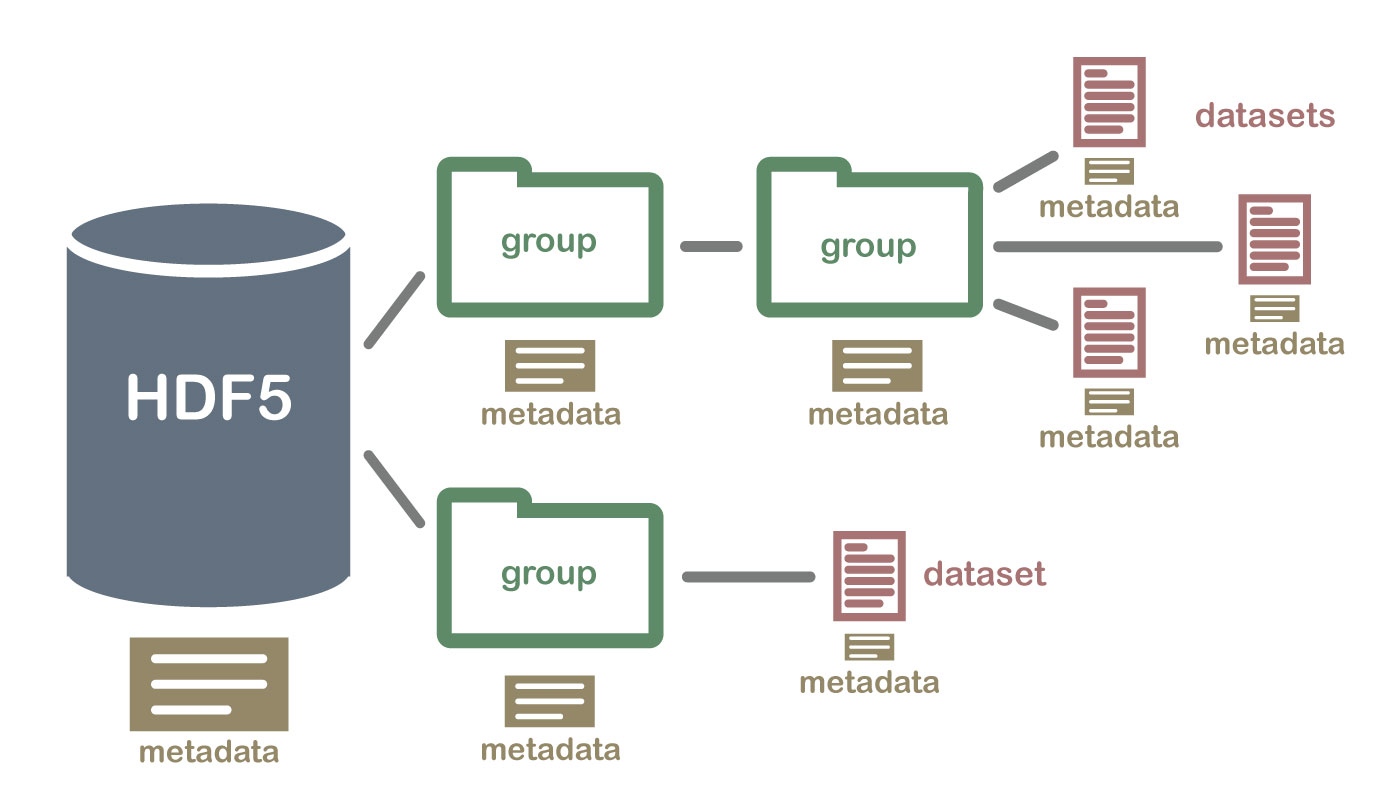
\includegraphics[width=\textwidth,height=0.6\textheight,keepaspectratio]{hdf5_structure.jpg}
    \end{center}
    \footnotetext{\href{https://www.neonscience.org/resources/learning-hub/tutorials/about-hdf5}{Source}}
\end{frame}
\begin{frame}[fragile]{HDF5}
    Unlike other frameworks in this section, the Python \lstinline[language=Python]{h5py} library operates similarly to the native Python's file I/O Operation.
    \begin{block}{Open and Close File}
        \begin{lstlisting}[language=Python]
file_obj = h5py.File(file_path, file_mode)
file_obj.close()
        \end{lstlisting}
    \end{block}
    \begin{block}{Writing and Reading Dataset}
        \begin{lstlisting}[language=Python]
file_obj.create_dataset(
dataset_path, shape=None,
dtype=None, data=None, **kwargs)
file_obj[dataset_path]
        \end{lstlisting}
    \end{block}
\end{frame}
\end{document}